% =====================================================================
% paper/thesis_ch5/sections/rebrac.tex
% §5.7 离线主线：双侧行为约束下的可部署性能（ReBRAC-Q 主结果 + 双机制消融）
% =====================================================================
% rev.1（2026-07-05）：§5.7 首版落地，依据已拍板方案
%   paper/thesis_ch5/section_5_7_rebrac_writing_plan.md（2026-07-05 定稿）执行。
%   结构：开篇段（承 §5.6.5 中心问题）→
%   §5.7.1 数据规模退化的翻转与基线差距（+23.0/+32.2pp、离散度不增、2000 不再劣于
%          1000、β1=4.0 ↔ α_BC≈0.25 公平对照锚）；
%   §5.7.2 可部署协议对特权协议参照的逼近（Welch t=0.104/p=0.9195、配对自助
%          Δ=+0.0060 CI[−0.030,+0.042]、差距闭合 53.0%/48.5%/57.6%、特权在主线上
%          退为难例种子救援 +12pp）；
%   §5.7.3 机制之一：价值侧支持惩罚跨数据集必要性（β2=0：−2.4pp/−5.0pp 同种子、
%          Q 漂移 −8.25→−0.13(+98%) / +15.22→+22.30(+46%)、难例种子 −17pp、
%          与特权救援构成双向闭环）；
%   §5.7.4 机制之二：层归一化独立必要（LN-off 2 种子 0.740±0.255、−16.2pp、
%          std×12、Q 反向漂 −12.09、单种子 −36pp；存在性结论）；
%   §5.7.5 对中心命题的含义与结论边界（正向轴前半 + 特权非必需 + finalist
%          稳健性优选埋点 + §5.8 伏笔散文式）；
%   §5.7.m 实施细节与可复现性（超参表 / 筛查→正式 / 统计检验全式 / 难例种子
%          具名一次 / 诚实 caveat 集中）。
%   数字逐项回查 docs/rebrac_experiment_report.md rev.8（§7.7 crosscomp 主对照 /
%   §7.10.3–.5 worldcomp deployable / §7.12.3–.8 privileged 5-seed / §7.13–§7.14
%   β2 消融 / §7.15 LN-off / §7.16 统计检验），TD3+BC 特权 per-seed 取
%   docs/rebrac_statistical_test_followup.md §1（聚合 0.922±0.086 已核对一致），
%   超参对照 paper/sections/appendix.tex App B + auv_nav/rebrac.py。未凭记忆、
%   未照抄 paper 1 表格数字。
%   ⚠ std 口径 = 报告刊值（0.902±0.021 / 0.672±0.045 一系，与 §5.6 同口径），
%     不用 paper 1 experiments.tex 的 Bessel 换算样本 std（0.902±0.024 一系）。
%   ⚠ worldcomp β2=0 按报告同种子口径写（0.960→0.910，−5.0pp）并写清对照基准，
%     不用 paper 1 的 5-seed 直比 −1.8pp。
%   ⚠ ReBRAC dep 0.928 vs TD3+BC dep 0.858（+7.0pp）与 2000>1000（0.918 对
%     0.902）均未做显著性检验且离散度可观，正文以点估计/定性表述，不写"显著高于"。
%   红线守：① LN 不进"可有可无"清单（−16.2pp 远超 β2=0 的 −2.4pp，§5.7.4 落地）；
%   ② mean 归因仅在 β1 vs β2 之间；③ LN n=2 仅存在性结论、不做重要性排序；
%   ④ 不写"+23–32pp 来自 actor anchor"——α_BC≈1/β1 换算落地后明确归于配方其余
%   部分整体（价值侧惩罚+层归一化+Q 归一化），不归单一轴；⑤ 零 §5.8 内容（临界
%   工况/N2' 零出现），伏笔散文式、不 \ref、不预报结果；持平表述用"未检测到统计
%   显著差异"（§5.3.6 口径），不写"超过"。
%   术语：全文 ReBRAC-Q（只引 §5.4 公式、零重复）；禁 teacher——0.990 写"采集器
%   自身成功率/参照水平"（承 §5.6）；gap closure→差距闭合比例；异策略；策略网络
%   (actor)/价值网络(critic)；工况；弯引号；难例种子正文匿名、seed 44 仅 §5.7.m
%   具名一次（图中自然可见）；"峰值"留 §5.5 专义，本节用"单点最高值"。
%   图：fig_ch5_rebrac_dotplot（worldcomp 三协议 per-seed 点图，mainline_edge
%   #2F5A6E 首次启用）/ fig_ch5_rebrac_qdrift（β2 消融 Q 漂移跨数据集一致性）；
%   均为 _ch5_style 重绘，不直搬 paper 1 fig2/fig3。paper 1 per-seed 特权对照表
%   （Tab 4）不进正文，分布由点图承载。本节无新增 cite。
%
% rev.2（2026-07-05）：独立对抗复审落地（数字忠实 / 论证统计 / 语体跨节 / 图表规范
%   四视角；数字逐项对 report rev.8 + followup §1 + 源码/驱动脚本独立重验）。
%   [CRIT-数字] 超参表 γ 0.995→0.99：rebrac.py:38 默认 0.99、两驱动脚本
%     GAMMA:-0.99、主线 notebook 零覆盖、TD3+BC 侧同为 0.99（口径对称）；0.995 系
%     paper 1 App B 笔误（疑自 SACConfig 抄串），rev.1 沿袭。声明句改"共同项与默认
%     一致、约束系数与训练预算为筛查所定"；表补梯度裁剪 10.0 与观测归一化两行。
%   [HIGH-数字] §5.7.4 单种子崩塌基线 0.920→0.890（report §7.15.4 自身笔误，与
%     §7.5 Stage C per-seed 表矛盾；report 已同步勘误），"36 个百分点"→"三十余"
%     （−33pp）。
%   [HIGH-论证] §5.7.3 双向闭环综合句撤"任一存在即可稳住"（worldcomp 可部署 β2
%     在位而难例种子仍 0.780，被本节自表反驳）→ 按 report §7.14.6 弱命题重写：
%     需某种价值侧稳定信号，crosscomp 由 β2 承担、worldcomp 须特权补足；§5.7.5
%     "同样的稳定化"限定为"均值层面所需的稳定化"。
%   [HIGH-跨节] §5.7.1 归因列表去 Q 归一化（§5.4.4 明言沿用 TD3+BC 写法、换算
%     恰以共享为前提）→ 配方差异 = 价值侧支持惩罚 + 层归一化；spec §0.4 红线 2
%     同步修正。
%   [HIGH-统计] "追平/相当"等价判断按 §5.3.6 承诺补实践容忍界：以本数据特权均值
%     抬升约 6pp 为最小实质效应，95%/99% 自助 CI 均落 ±6pp 内（99% [−4.2,+5.2]）。
%   [MED] std 口径说明入 §5.7.m（特权 ReBRAC-Q 0.026 为样本口径、总体约 0.023，
%     余为总体口径）；TD3+BC 特权自身低位种子 0.760 补一句（非同一颗、离散度未收
%     窄 0.086 对 0.080），"对全体种子的平均改善"→"均值层面整体抬升而非个别种子
%     救援"（§7.12.8 原口径）；"价值项重新带来净增益"降为"退化不再出现"（无去价
%     值项对照）；LN-off 补同种子口径锚（0.910→0.740，−17.0pp）；"全部实验单元
%     共用"→"主线实验单元"（消融单元单处改动）；致密支持集机制语气回 §5.6 hedge。
%   [LOW] "数据集不变的"→"在两类数据集上同向成立"；§5.7.m 闭合比例三值改自足
%     表述；点图注补"纵轴自 0.70 起"；"由该图承载/见结果文件"赘语清理；字典序
%     指针去重；表内"64（每轮…）"重复删。浮动漂移（表 5.10/图 5.12 漂 1–2 页）
%     属章级登记延后项（验收 F·M2），本轮不动。两图数据全对、脚本未动。
% =====================================================================

\section{离线主线：双侧行为约束下的可部署性能}\label{sec:ch5_rebrac}

\S\ref{subsec:ch5_td3bc_transition} 把离线基线的限制归结为数据支持集结构与可部署价值网络信息两个瓶颈，并留下一个中心问题：可部署单点观测下，离线性能能否借由策略与价值两侧的行为约束，逼近训练期接收特权观测的同类协议。本节以 \S\ref{subsec:ch5_method_rebrac} 定义的离线主线方法 ReBRAC-Q——Q 归一化双正则 TD3+BC 变体——正面回答这一问题。实验沿用与 \S\ref{sec:ch5_td3bc} 完全相同的口径：历史效率导向奖励（\S\ref{subsec:ch5_reward}）、亚临界主工况、可部署单点传感 $s_0$ 与 $k=4$ 历史堆叠；离线数据为横流补偿参照的一千与两千回合数据集，以及世界坐标系流速补偿参照的一千回合数据集（\S\ref{subsec:ch5_datasets}）。行为约束系数经小规模筛查锁定为 $(\beta_1,\beta_2)=(4.0,\,2.0)$ 后，各数据集上的主线实验单元共用这一配置，在正式协议下以五个随机种子训练、每种子在固定评估集上终检评估 $100$ 回合（\S\ref{subsec:ch5_eval}）；筛查流程与统计检验细节见 \S\ref{subsec:ch5_rebrac_impl}。沿这一协议展开的证据构成一条递进的线索：数据规模增大导致的退化被翻转、对基线的差距同时拉开；在暴露信息瓶颈的同一数据上，可部署协议追平了训练期接收特权观测的参照协议；随后的两项单变量消融把这一性能定位到价值侧支持惩罚与价值网络层归一化这两个各自必要、互不替代的构件上，并据此界定本节结论对中心命题的贡献与边界。

\subsection{数据规模退化的翻转与基线差距}\label{subsec:ch5_rebrac_scale}

沿 \S\ref{subsec:ch5_td3bc_support} 的同一条数据规模线索，ReBRAC-Q 在横流补偿参照的一千与两千回合数据集上给出的图景与单侧约束基线判然有别（表~\ref{tab:ch5_rebrac_main}）。一千回合数据上，终检成功率为 $0.902 \pm 0.021$，较 TD3+BC 同数据经后验选择最优行为克隆权重的 $0.672 \pm 0.045$ 提高 $23.0$ 个百分点；两千回合数据上为 $0.918 \pm 0.030$ 对 $0.596 \pm 0.036$，差距扩大到 $32.2$ 个百分点。跨随机种子离散度同时不增反降（$0.021$ 对 $0.045$、$0.030$ 对 $0.036$）：均值的大幅提升并未以方差放大为代价，而是均值与稳定性同向改善。

比幅度更能说明问题的是定性翻转。TD3+BC 与同预算纯行为克隆都在两千回合处可复现地回落（\S\ref{subsec:ch5_td3bc_support}），而 ReBRAC-Q 下两千回合不再低于一千回合，点估计反而略高（$0.918$ 对 $0.902$）。数据相同、支持集结构相同，回落却随行为约束形式而消失，这说明 \S\ref{subsec:ch5_td3bc_support} 界定的第一个瓶颈并非数据规模固有的惩罚：该处所指认的由确定性采集形成的高度集中的支持结构，超出的只是单侧行为约束的消化能力，仍在双侧约束的消化能力之内。数据支持集结构的约束由此显示出算法相对性——它约束的是把全部数据信息压在单一模仿项上的方法，而非离线学习本身。

这一对照的公平性可以从系数换算上精确界定。\S\ref{subsec:ch5_method_rebrac} 曾指出，$\beta_1$ 与 TD3+BC 的 $\alpha_{\mathrm{BC}}$ 只有在 Q 归一化写法下才存在近似换算：把 \eqref{eq:ch5_rebrac_actor} 整体除以 $\beta_1$，即得与 \eqref{eq:ch5_td3bc_actor} 同形的单位化形式，策略侧锚定强度对应 $\alpha_{\mathrm{BC}} \approx 1/\beta_1$。本节配置 $\beta_1 = 4.0$ 对应 $\alpha_{\mathrm{BC}} \approx 0.25$，恰与 TD3+BC 在一千回合数据上经后验选择的最优权重 $\alpha_{\mathrm{BC}} = 0.25$ 重合：两方法把策略输出拉向数据动作的强度处在同一水平，二十余个百分点的差距便不能归于策略侧锚定强度的再调节，而来自配方其余部分——价值侧支持惩罚与价值网络层归一化——的整体作用；Q 归一化为两方法共享的写法，正是它使上述换算得以成立。这两个成分各自的贡献并不均匀，也不宜笼统合并成单一解释，本节稍后以两项单变量消融分别界定。

\begin{table}[t]
\centering
\caption{离线主线 ReBRAC-Q 与行为约束基线 TD3+BC 的主对照（历史效率导向奖励、亚临界工况、$s_0$ 单点传感、$k=4$ 历史堆叠；正式五随机种子协议、每种子终检评估 $100$ 回合，成功率为均值 $\pm$ 跨随机种子标准差）。ReBRAC-Q 全部单元共用同一配置 $(\beta_1,\beta_2)=(4.0,\,2.0)$；TD3+BC 各行为该数据与协议下经后验选择的最优行为克隆权重（承 \S\ref{sec:ch5_td3bc}）。可部署协议与特权协议的差异仅在价值网络训练期可见的信息（\S\ref{subsec:ch5_method_protocol}）；采集器一行为世界坐标系流速补偿参照自身轨迹的成功率，作为该数据上的参照水平。世界坐标系流速补偿参照数据上两方法的统计比较见正文与 \S\ref{subsec:ch5_rebrac_impl}。}
\label{tab:ch5_rebrac_main}
\setlength{\tabcolsep}{5pt}
\begin{tabular}{l l c c c}
\toprule
\textbf{数据集} & \textbf{协议} & \textbf{最优 $\alpha_{\mathrm{BC}}$} & \textbf{TD3+BC} & \textbf{ReBRAC-Q} \\
\midrule
横流补偿参照（$1000$ 回合） & 可部署 & $0.25$ & $0.672 \pm 0.045$ & $\mathbf{0.902 \pm 0.021}$ \\
横流补偿参照（$2000$ 回合） & 可部署 & $0.15$ & $0.596 \pm 0.036$ & $\mathbf{0.918 \pm 0.030}$ \\
\addlinespace
\multirow{2}{*}{\makecell[l]{世界坐标系流速补偿参照\\（$1000$ 回合）}} & 可部署 & $\to 0$（纯行为克隆） & $0.858 \pm 0.080$ & $0.928 \pm 0.077$ \\
 & 特权 & $0.1$ & $0.922 \pm 0.086$ & $0.934 \pm 0.026$ \\
\addlinespace
采集器（参照水平） & --- & --- & \multicolumn{2}{c}{$0.990$} \\
\bottomrule
\end{tabular}
\end{table}

\subsection{可部署协议对特权协议参照的逼近}\label{subsec:ch5_rebrac_worldcomp}

世界坐标系流速补偿参照的一千回合数据把考察从数据规模转向价值网络的信息，即 \S\ref{subsec:ch5_td3bc_critic} 暴露第二个瓶颈的同一数据。该数据上 TD3+BC 的可部署最优配置退回纯行为克隆（$0.858 \pm 0.080$）；ReBRAC-Q 在可部署协议下保持价值改进项工作，终检成功率 $0.928 \pm 0.077$，相对纯行为克隆水平的点估计提高 $7.0$ 个百分点——单侧约束下“价值项无益于可部署策略”的退化，在双侧约束下不再出现。更强的结论来自与特权协议参照的直接比较：可部署 ReBRAC-Q 的 $0.928 \pm 0.077$ 与训练期接收特权观测的 TD3+BC 的 $0.922 \pm 0.086$ 之间，以随机种子为推断单位的 Welch 检验不拒绝均值相等（$t = 0.104$，双侧 $p = 0.9195$），回合级配对自助复核给出的均值差点估计 $+0.006$、$95\%$ 置信区间 $[-0.030,\ +0.042]$ 跨越零（\S\ref{subsec:ch5_eval} 口径）：两者未检测到统计显著差异。本章对“性能相当”类判断的附加要求（\S\ref{subsec:ch5_eval}）在此按如下容忍界兑现：以该数据上训练期特权观测所带来的约 $6$ 个百分点均值级抬升（\S\ref{subsec:ch5_td3bc_critic}）为具有实质意义的最小效应量，两协议均值差的 $95\%$ 与 $99\%$ 自助置信区间（后者见 \S\ref{subsec:ch5_rebrac_impl}）均整体落在 $\pm 6$ 个百分点之内。\S\ref{subsec:ch5_td3bc_transition} 留下的中心问题由此得到肯定回答——双侧行为约束使可部署价值网络无须任何部署期不可得的信息，即可给出与特权协议参照相当的改进信号。

以差距闭合比例衡量（定义见 \S\ref{subsec:ch5_rebrac_impl}），可部署 ReBRAC-Q 把 TD3+BC 可部署协议与采集器自身成功率 $0.990$ 之间约 $13$ 个百分点的差距闭合 $53.0\%$，点估计略高于 TD3+BC 特权协议的 $48.5\%$；受随机种子数量所限，闭合比例之差只宜作方向性观察，其置信区间在 \S\ref{subsec:ch5_rebrac_impl} 如实给出。采集器自身成功率在此仍只充当该数据上的高质量参照水平，衡量与数据来源之间尚存的余量。

把特权协议施加到 ReBRAC-Q 自身，特权观测的作用形态随之改变（图~\ref{fig:ch5_rebrac_dotplot}）。价值网络在训练期补入等效来流估计后，成功率为 $0.934 \pm 0.026$，均值仅比可部署协议高 $0.6$ 个百分点——在离线主线方法上，特权观测不再带来均值层面的抬升。它的残余作用集中于单一难例种子：该种子在可部署协议下是五个随机种子中唯一低于 $0.9$ 的离群点（$0.780$），特权协议将其救回 $0.900$（$+12$ 个百分点），其余种子保持原位或轻微下移；种子级离散度相应由 $0.077$ 收窄至 $0.026$。特权信息的价值由此从均值改进退化为对个别优化失稳的种子级救援。

\begin{figure}[t]
    \centering
    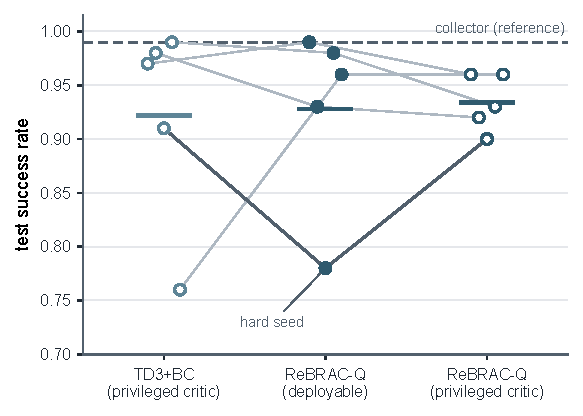
\includegraphics[width=96mm]{figures/fig_ch5_rebrac_dotplot.pdf}
    \caption{世界坐标系流速补偿参照数据（亚临界工况、历史效率导向奖励、$s_0$ 单点传感、$k=4$ 历史堆叠）上三种协议的种子级终检成功率（五随机种子、每种子 $100$ 回合；纵轴自 $0.70$ 起；细线连接同一随机种子，短横杠为各协议均值，虚线为采集器自身成功率 $0.990$ 的参照水平；实心点为可部署协议，空心点为特权协议）。可部署协议下的 ReBRAC-Q（中列）与训练期接收特权观测的 TD3+BC（左列）处于同一水平，二者未检测到统计显著差异（正文）；把特权协议施加到 ReBRAC-Q 自身（右列）几乎不改变均值，其作用集中于把可部署协议下唯一的难例种子（深色连线，图中标注 hard seed）由 $0.780$ 救回 $0.900$，其余种子保持原位或轻微下移。}
    \label{fig:ch5_rebrac_dotplot}
\end{figure}

与 \S\ref{subsec:ch5_td3bc_critic} 的观察并置，特权观测的作用形态随算法而变。在单侧约束的 TD3+BC 上，训练期特权观测对应约 $6$ 个百分点的均值级抬升，其显著性虽未确立，形态上呈现为均值层面的整体抬升而非集中于个别种子的救援——特权协议下的 TD3+BC 自身仍留有一个低位种子（$0.760$，与 ReBRAC-Q 的难例种子并非同一颗，图~\ref{fig:ch5_rebrac_dotplot} 左列可见），种子间离散度并未收窄（$0.086$ 对可部署协议的 $0.080$）。在双侧约束的 ReBRAC-Q 上，均值抬升消失，只余对单一离群种子的救援与种子间离散度的收窄。训练期特权信息是否有用，由此并非观测协议的固有属性，而取决于算法把可部署信息利用到何种程度——价值侧支持惩罚已经完成的稳定化，特权观测便无须重复。这一结论锚定于亚临界工况、世界坐标系流速补偿参照数据的离线设定之内，不外推到其它工况、其它数据来源或在线情形。

\subsection{机制之一：价值侧支持惩罚的跨数据集必要性}\label{subsec:ch5_rebrac_beta2}

双侧约束中的价值侧支持惩罚是否确在起作用，由 $\beta_2 = 0$ 的单变量消融回答（表~\ref{tab:ch5_rebrac_beta2}）。横流补偿参照一千回合数据上，关闭价值侧惩罚使五随机种子的成功率由 $0.902$ 降至 $0.878 \pm 0.090$（$-2.4$ 个百分点）；世界坐标系流速补偿参照数据上，两随机种子的低成本探查在与完整配置相同的一对种子上由 $0.960$ 降至 $0.910$（$-5.0$ 个百分点；对照基准为完整配置在同一对种子上的均值，而非五种子均值）。仅就均值而论，损失有限，价值侧惩罚看似可有可无。

训练侧诊断给出相反的图景（图~\ref{fig:ch5_rebrac_qdrift}）。以训练后期窗口内的平均自举目标衡量价值估计的保守程度（读取口径见 \S\ref{subsec:ch5_rebrac_impl}），两个数据集的完整配置基线恰好位于零的两侧：横流补偿参照数据上为 $-8.25$，世界坐标系流速补偿参照数据上为 $+15.22$。移除价值侧惩罚后，二者朝同一方向漂移 $+7$ 至 $+8$ 个绝对单位——前者由 $-8.25$ 漂至 $-0.13$（相对幅度约 $+98\%$），后者由 $+15.22$ 漂至 $+22.30$（约 $+46\%$）——即都朝更不保守的方向移动。基线符号相反而漂移方向与幅度一致，表明该惩罚抑制价值自举外推的机制不依赖具体数据集的价值尺度与符号，在两类数据集上同向成立；成功率均值上的“小损失”低估了它在自举链路中承担的稳定作用。

\begin{table}[t]
\centering
\caption{价值侧支持惩罚的单变量消融（$\beta_2 = 0$，其余配置不变，可部署协议）。成功率为终检评估均值（多种子时附跨随机种子标准差）；自举目标 $Q$ 为训练后期窗口内的平均自举目标（诊断量，读取自价值侧惩罚施加之前，\S\ref{subsec:ch5_rebrac_impl}）。世界坐标系流速补偿参照数据上的 $\beta_2 = 0$ 单元为两随机种子探查，其成功率的同种子对照基准为完整配置在同一对种子上的均值 $0.960$（正文）；该行完整配置的 $0.928 \pm 0.077$ 与自举目标 $+15.22$ 为五种子值。}
\label{tab:ch5_rebrac_beta2}
\setlength{\tabcolsep}{5pt}
\begin{tabular}{l l c c c}
\toprule
\textbf{数据集} & \textbf{配置} & \textbf{种子数} & \textbf{成功率} & \textbf{自举目标 $Q$} \\
\midrule
\multirow{2}{*}{横流补偿参照（$1000$ 回合）} & $\beta_2 = 2.0$（完整） & $5$ & $0.902 \pm 0.021$ & $-8.25$ \\
 & $\beta_2 = 0$ & $5$ & $0.878 \pm 0.090$ & $-0.13$ \\
\addlinespace
\multirow{2}{*}{\makecell[l]{世界坐标系流速补偿参照\\（$1000$ 回合）}} & $\beta_2 = 2.0$（完整） & $5$ & $0.928 \pm 0.077$ & $+15.22$ \\
 & $\beta_2 = 0$ & $2$ & $0.910$ & $+22.30$ \\
\bottomrule
\end{tabular}
\end{table}

\begin{figure}[t]
    \centering
    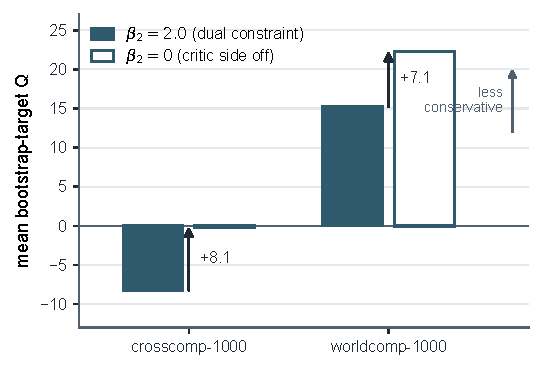
\includegraphics[width=90mm]{figures/fig_ch5_rebrac_qdrift.pdf}
    \caption{移除价值侧支持惩罚（$\beta_2 = 0$）后自举目标 $Q$ 的跨数据集同向漂移。纵轴为训练后期窗口内的平均自举目标（诊断量，读取自价值侧惩罚施加之前，\S\ref{subsec:ch5_rebrac_impl}）。横流补偿参照数据（图中 crosscomp-1000）与世界坐标系流速补偿参照数据（图中 worldcomp-1000）的完整配置基线（实心柱）位于零的两侧，移除该惩罚（空心柱）后二者都朝更不保守的方向漂移 $+7$ 至 $+8$ 个绝对单位（箭头），相对幅度分别约 $+98\%$ 与 $+46\%$。横流补偿参照数据的消融为五随机种子，世界坐标系流速补偿参照数据的为两随机种子探查。}
    \label{fig:ch5_rebrac_qdrift}
\end{figure}

均值变化有限的另一面，是离群种子的崩塌。\S\ref{subsec:ch5_rebrac_worldcomp} 中被特权协议救回的同一难例种子，在横流补偿参照数据上失去价值侧惩罚后由 $0.870$ 跌至 $0.700$（$-17$ 个百分点），其余种子仅在数个百分点内小幅波动——五种子均值 $-2.4$ 个百分点的损失几乎全部由这一个种子贡献，消融后离散度由 $0.021$ 放大至 $0.090$ 亦源于此。与 \S\ref{subsec:ch5_rebrac_worldcomp} 的观察合并，同一难例种子构成一组双向对照：世界坐标系流速补偿参照数据上，向价值网络补入特权观测将其救回；横流补偿参照数据上，移除价值侧惩罚将其压垮。两处证据来自不同的数据集，其方向却一致：仅靠策略侧锚定不足以稳住该种子，它在两个数据集上都需要某种价值侧的稳定信号——这一信号在横流补偿参照数据上由价值侧支持惩罚承担（移除即崩），在世界坐标系流速补偿参照数据上则不足以由支持惩罚单独提供、须由训练期特权观测补足（补入方救回）。该种子的失稳系统性地跟随价值侧稳定信号的有无而出现与消失，这使“难例种子的波动只是统计噪声”的解释难以成立；至于稳定信号本身，横流补偿参照数据上的对照表明它可以完全不依赖特权信息而由双侧约束提供。

\subsection{机制之二：层归一化与双侧惩罚是独立必要构件}\label{subsec:ch5_rebrac_ln}

价值网络的层归一化在 \S\ref{subsec:ch5_method_rebrac} 被定位为表征稳定性的基础设施，其必要性由关闭层归一化的两种子探查检验（表~\ref{tab:ch5_rebrac_ablation}）。横流补偿参照一千回合数据上保持 $(\beta_1,\beta_2)=(4.0,\,2.0)$ 不变、仅移除价值网络层归一化后，两种子成功率均值跌至 $0.740 \pm 0.255$，相对完整配置的五种子均值低 $16.2$ 个百分点（同一对种子上完整配置的均值为 $0.910$，同种子口径的差距为 $17.0$ 个百分点），跨种子离散度由 $0.021$ 放大约 $12$ 倍；两种子中一个基本保持原有水平（$0.920$），另一个由 $0.890$ 崩至 $0.560$，呈现训练层面的完全失稳。这一三十余个百分点的单种子崩塌在关闭价值侧惩罚的消融中从未出现——同一种子在 $\beta_2 = 0$ 下仍有 $0.920$——层归一化缺失引入的是一类此前未曾观察到的失稳模式。

训练侧诊断进一步把两项消融区分开。移除价值侧惩罚使自举目标朝更不保守的方向漂移（$+8.12$ 个单位）；移除层归一化则使其反向漂向更负（$-8.25$ 至 $-12.09$），并伴随种子间方差的爆发。一个朝乐观外推、一个朝表征失稳，两种退化方向相反、形态各异、出现在不同的种子上，互不替代——层归一化与价值侧支持惩罚是两个独立的必要构件，而非同一机制的两种呈现。

结论强度须与证据规模相称。层归一化消融仅两随机种子，它支撑的是“层归一化是离线价值学习的必要构件”这一存在性结论，不支撑层归一化与双侧惩罚之间的重要性排序；均值层面的归因比较也只在策略侧 $\beta_1$ 与价值侧 $\beta_2$ 两个行为约束系数之间成立，不外推为对配方全体成分的分解。同时，$16.2$ 个百分点的退化远超 $\beta_2 = 0$ 的 $2.4$ 个百分点，这从反面划清了一条界线：层归一化不属于“可有可无”的附加能力，而是 \S\ref{subsec:ch5_method_rebrac} 所定位的运行前提，与“训练期特权观测是否必需”这一命题维度相互正交——移除它损害的是价值学习本身，而非某种可选信息来源。

\begin{table}[t]
\centering
\caption{价值侧惩罚与层归一化的三向对照（横流补偿参照一千回合数据、可部署协议；每行相对完整配置只改动一处）。成功率为终检评估均值 $\pm$ 跨随机种子标准差；自举目标 $Q$ 为训练后期窗口内的平均自举目标及其相对完整配置的漂移。$\Delta$ 均值以完整配置的五种子均值为基准，两种子单元的同种子口径对照见正文。层归一化消融为两随机种子探查，仅支撑必要构件的存在性结论（正文）。}
\label{tab:ch5_rebrac_ablation}
\setlength{\tabcolsep}{5pt}
\begin{tabular}{l c c c c}
\toprule
\textbf{配置} & \textbf{种子数} & \textbf{成功率} & \textbf{$\Delta$ 均值} & \textbf{自举目标 $Q$（漂移）} \\
\midrule
完整配置 $(\beta_1{=}4.0,\ \beta_2{=}2.0)$ & $5$ & $0.902 \pm 0.021$ & --- & $-8.25$ \\
关闭价值侧惩罚（$\beta_2 = 0$） & $5$ & $0.878 \pm 0.090$ & $-2.4$~pp & $-0.13$（$+8.12$，朝乐观） \\
关闭价值网络层归一化 & $2$ & $0.740 \pm 0.255$ & $-16.2$~pp & $-12.09$（$-3.84$，朝更负） \\
\bottomrule
\end{tabular}
\end{table}

\subsection{对中心命题的含义与结论边界}\label{subsec:ch5_rebrac_implications}

本节结果落在中心命题的正向一侧。双侧行为约束没有为系统增添任何能力——不增加空间传感器、不向价值网络注入特权观测、不引入更具表达力的策略先验——它所做的只是把既有数据用得更充分：策略侧继续以原始数据动作为模仿目标，价值侧让自举不越出同一份数据的支持。就本节的高质量确定性采集数据而言，以原始动作为模仿目标工作良好，“模仿目标与数据质量相适配”这一正向途径的前半在此得到正面例证；当数据条件变化时这一模仿目标是否仍然恰当，属于算法与数据条件的交互问题，留待算法比较的一节考察。

反向一侧，“向价值网络注入特权观测”在离线主线方法上退为非必需。均值层面，特权协议不再带来可检测的抬升；其残余价值收缩为对单一难例种子的救援。本章并不因此断言特权信息无用——难例种子的救援是真实的，\S\ref{subsec:ch5_rebrac_beta2} 的双向对照也确认价值侧信息通道本身有效——但在部署约束下，均值层面所需的稳定化可由不依赖特权信息的价值侧支持惩罚完成，特权观测便不再是可部署离线性能的先决条件。这与 \S\ref{sec:ch5_td3bc} 的图景合并成一个条件化的判断：训练期特权观测的必要性随算法对既有信息的利用程度而消长，算法侧的改进空间未用尽之前，为价值网络增添信息并非唯一的、也未必是首选的杠杆。

界定本节结论的还有两个边界。所选配置 $(\beta_1{=}4.0,\ \beta_2{=}2.0)$ 是跨种子稳健性的优选而非单点最高值的优选：筛查网格中锚定更弱的配置曾在个别种子上取得更高的单点成功率，该配置的胜出来自把在弱锚定下系统性偏弱的难例种子稳定收回；后文讨论行为约束强度在不同设定间的关系时，须以这一选择标准为口径。此外，本节全部结果限于亚临界工况、历史效率导向奖励与横流穿越几何之内；双侧行为约束下的可部署性能在更强流动工况下能否保持，是下一节泛化边界考察的对象。

\subsection{实施细节与可复现性}\label{subsec:ch5_rebrac_impl}

本节沿用 \S\ref{subsec:ch5_method_impl} 的网络结构、优化器与检查点选择规则；表~\ref{tab:ch5_rebrac_hparams} 汇总所用 ReBRAC-Q 配置的完整超参数：网络、优化器与确定性分支共同项的取值与实现中的配置默认值一致，行为约束系数与训练预算则为筛查所定、经命令行显式设定。三个离线数据集的采集协议与转移规模见 \S\ref{subsec:ch5_datasets} 与 \S\ref{subsec:ch5_impl}；正式协议每种子训练 $64$ 个训练轮次（epoch），每轮完整遍历离线数据集一次，检查点每 $8$ 轮保存一次，在验证集（$40$ 回合）上按 \S\ref{subsec:ch5_method_impl} 的字典序规则选择，终检评估 $100$ 回合。

\begin{table}[t]
\centering
\caption{ReBRAC-Q 实验配置的完整超参数（本节主线实验单元共用，消融单元在此基础上仅作正文所述的单处改动；符号承 \S\ref{sec:ch5_methodology}）。}
\label{tab:ch5_rebrac_hparams}
\setlength{\tabcolsep}{5pt}
\begin{tabular}{l l}
\toprule
\textbf{项目} & \textbf{取值} \\
\midrule
网络结构 & 策略与价值网络均为三隐层 $256$ 单元 MLP（ReLU） \\
层归一化 & 价值网络每层后接层归一化；策略网络不用 \\
观测归一化 & 按离线数据集观测统计量标准化（数值下界 $10^{-3}$） \\
行为约束系数 & $\beta_1 = 4.0$（策略侧）、$\beta_2 = 2.0$（价值侧） \\
Q 归一化下界 $\varepsilon$ & $10^{-6}$ \\
目标平滑噪声 $\sigma$ / 截断 $c$ & $0.2$ / $0.5$ \\
延迟策略更新 & 每 $2$ 次价值网络更新执行 $1$ 次策略更新 \\
优化器与学习率 & Adam，策略与价值网络均 $3 \times 10^{-4}$ \\
梯度裁剪范数 & $10.0$ \\
折扣因子 $\gamma$ / 软更新系数 $\tau$ & $0.99$ / $0.005$ \\
批量大小 & $256$ \\
训练轮次 & $64$ \\
检查点保存 / 验证 / 终检 & 每 $8$ 轮一次 / $40$ 回合 / $100$ 回合 \\
随机种子 & 固定 $5$ 个（\S\ref{subsec:ch5_eval}） \\
\bottomrule
\end{tabular}
\end{table}

行为约束系数的筛查在横流补偿参照的一千与两千回合数据上进行：网格 $\beta_1 \in \{1.0,\,2.0,\,4.0\} \times \beta_2 \in \{1.0,\,2.0\}$，每格三随机种子、测试 $40$ 回合。$(4.0,\,2.0)$ 在两个数据集上同时以均值与离散度胜出后，升入正式五随机种子、每种子终检评估 $100$ 回合的协议；世界坐标系流速补偿参照数据直接沿用该配置、不再重扫——Q 归一化使价值改进项的尺度随数据集自适应，$\beta_1$ 的取值因此可跨数据集迁移。筛查中的跨随机种子超参数后验选择按 \S\ref{subsec:ch5_method_impl} 的同一字典序验证指标执行。

统计检验的完整形式如下。Welch 不等方差 $t$ 检验以两组各五个种子级成功率均值为样本，自由度按 Welch--Satterthwaite 公式计算（本节主对照 $t = 0.104$、自由度约 $7.9$、双侧 $p = 0.9195$）。回合级配对自助以两协议共用的同一固定评估集的 $100$ 个评估回合为重采样单位，每个回合先取跨种子成功率均值再作 $B = 10^4$ 次有放回重采样，报告均值差的百分位置信区间：$95\%$ 区间 $[-0.030,\ +0.042]$、$99\%$ 区间 $[-0.042,\ +0.052]$，双侧自助 $p \approx 0.776$。差距闭合比例定义为（方法成功率 $-$ 可部署基线成功率）$/$（采集器自身成功率 $-$ 可部署基线成功率），其中可部署基线取 TD3+BC 可部署协议的 $0.858$、采集器自身成功率为 $0.990$；本节引用的 $53.0\%$、$48.5\%$ 与 $57.6\%$（依次对应可部署协议 ReBRAC-Q、特权协议 TD3+BC 与特权协议 ReBRAC-Q）均为该定义下的点估计，闭合比例之差的种子级自助 $95\%$ 置信区间极宽且跨越零（约 $[-62,\ +86]$ 个百分点），故闭合比例的比较只作方向性描述。训练侧诊断量“自举目标 $Q$”读取自价值侧惩罚施加之前的自举目标，在训练后期约四分之一的更新窗口内取均值。

正文所称难例种子为固定种子组中的 seed~$44$；筛查网格中 $\beta_1 \le 2.0$ 的全部配置下它几乎总是最弱的种子，其系统性困难先于本节全部消融而存在；种子级分布见图~\ref{fig:ch5_rebrac_dotplot}，原始逐种子记录保留于复现实验配置与结果记录。诚实限定集中登记于此。世界坐标系流速补偿参照数据上的 $\beta_2 = 0$ 探查仅两随机种子，且刻意不含难例种子（以先验证典型种子的机制方向），故该数据上难例种子失去价值侧惩罚后的行为未测；层归一化消融同为两随机种子，仅支撑存在性结论。TD3+BC 在世界坐标系流速补偿参照数据上的对照训练预算为 $96$ 轮、ReBRAC-Q 为 $64$ 轮，各按其自身验证协议选定；预算差异的方向不利于 ReBRAC-Q，故不影响持平结论的方向，但在此如实登记。表中标准差沿用实验报告刊值：世界坐标系流速补偿参照数据上特权协议 ReBRAC-Q 的 $0.026$ 为样本标准差口径（按总体口径约为 $0.023$），其余单元均为总体口径，两种口径不改变本节任何比较的方向。五个随机种子对 $0.6$ 个百分点量级的均值差异检验功效很低，“未检测到统计显著差异”的表述正以此为界——它量化的是在该样本规模下两协议不可区分，而非证明两者严格相等。
